%%%%%%%%%%%%%%%%%%%%%%%%%%%%%%%%%%%%%%%%%%%%%%%%%%%%%%%%%%%%%%%%%%%%%%%%%%%%
%% Trim Size: 9.75in x 6.5in
%% Text Area: 8in (include Runningheads) x 5in
%% ws-ijait.tex   :   01-10-2014
%% Tex file to use with ws-ijait.cls written in Latex2E.
%% The content, structure, format and layout of this style file is the
%% property of World Scientific Publishing Co. Pte. Ltd.
%%%%%%%%%%%%%%%%%%%%%%%%%%%%%%%%%%%%%%%%%%%%%%%%%%%%%%%%%%%%%%%%%%%%%%%%%%%%
%%

\documentclass{ws-ijait}

\usepackage{epstopdf}
\usepackage{color}
\usepackage{xspace}
\usepackage{booktabs}

\usepackage[vlined,ruled,norelsize]{algorithm2e}


\begin{document}

\newcommand{\red}[1]{{\color{red} #1}}

\markboth{Tom\'a\v{s} K\v{r}en, Martin Pil\'at, Roman Neruda}
{Strongly Typed Genetic Programming for Automatic Creation of Machine-Learning
Workflows}

%%%%%%%%%%%%%%%%%%%%% Publisher's Area please ignore %%%%%%%%%%%%%%%
%
\catchline{}{}{}{}{}
%
%%%%%%%%%%%%%%%%%%%%%%%%%%%%%%%%%%%%%%%%%%%%%%%%%%%%%%%%%%%%%%%%%%%%

\title{Automatic Creation of Machine-Learning Workflows with Strongly Typed
Genetic Programming}


\author{Tom\'a\v{s} K\v{r}en}

\address{Charles University, Faculty of Mathematics and Physics, Malostransk\'e
n\'am\v{e}st\'i 25, 118 00 Prague, Czech Republic, Tomas.Kren@mff.cuni.cz}

\author{Martin Pil\'at}
\address{Charles University, Faculty of Mathematics and Physics, Malostransk\'e
n\'am\v{e}st\'i 25, 118 00 Prague, Czech Republic, Martin.Pilat@mff.cuni.cz}


\author{Roman Neruda}
\address{Institute of Computer Science, The Czech Academy of Sciences, 
Pod Vod\'arenskou v\v{e}\v{z}\'i 271/2, 182 07 Prague, Czech Republic, 
roman@cs.cas.cz}

\newcommand{\ar}{\rightarrow}
\newcommand{\Dlong}{unlabeled data\xspace}
\newcommand{\LDlong}{labeled data\xspace}
\newcommand{\Dshort}{\textit{$D$}\xspace}
\newcommand{\LDshort}{\textit{$LD$}\xspace}
\newcommand{\dia}{\textit{$ens_1$}\xspace}
\newcommand{\diaZero}{\textit{$ens_0$}\xspace}
\newcommand{\splitComb}{\textit{$split$}\xspace}
\newcommand{\cons}{\textit{$cons$}\xspace}

\newcommand{\komb}[1]{\textit{#1}}
\newcommand{\kons}[1]{\textit{#1}}

\newcommand{\Dag}{\kons{Dag}}
\newcommand{\D}{\kons{D}}
\newcommand{\LD}{\kons{LD}}
\newcommand{\Boo}{\kons{Boo}}
\newcommand{\V}{\kons{V}}
\newcommand{\Succ}{\kons{S}}
\newcommand{\Zero}{\kons{0}}
\newcommand{\Same}{\kons{Same}}
\newcommand{\Disjoint}{\kons{Disjoint}}

\newcommand{\Suc}[1]{(\Succ\ #1)}
\newcommand{\Ve}[3]{(\V\ #1\ #2\ #3)}

\newcommand{\DAG}[2]{(\Dag\ #1\ #2)}
\newcommand{\splitter}[4]{\DAG{#1}{\Ve{#2}{#3}{#4}}}
\newcommand{\merger}[4]{\DAG{\Ve{#1}{#3}{#4}}{#2}}
\newcommand{\dvaPlus}[1]{\Suc{\Suc{#1}}}
\newcommand{\dva}{\dvaPlus{\Zero}}



\newcommand{\la}{\leftarrow\xspace}
\newcommand{\op}{\operatorname}
\newcommand{\mgu}[1]{\op{MGU}(#1)}


\newcommand{\Pseudokod}[4]{
	\begin{figure}[!t]
	\removelatexerror
	\begin{algorithm}[H]
		\caption{\label{#4}#1}
		\DontPrintSemicolon
		\SetKwProg{Fn}{function}{}{}
		\Fn{#2}{#3}
	\end{algorithm}
	\end{figure}
}

\makeatletter
\newcommand{\removelatexerror}{\let\@latex@error\@gobble}
\makeatother

\maketitle

\begin{history}
\received{(Day Month Year)}
\revised{(Day Month Year)}
\accepted{(Day Month Year)}
%\comby{(xxxxxxxxxx)}
\end{history}

\begin{abstract}
\end{abstract}

\keywords{Genetic programming; machine learning workflows; asynchronous
evolutionary algorithm}

\section{Introduction}	

\section{Related Work}


\section{Our approach}




\subsection{Individual representation}

\subsubsection{What is a machine learning workflow?}
Let us start with brief clarification of what we mean by term machine learning workflow. We can distinguish two kinds of machine learning methods: basic and combined. The basic methods are particular \textit{named} methods such as specific classification, regression, clustering, preprocessing or voting algorithms. On the other hand, the combined methods are \textit{anonymous} results of combining several basic methods into one compound by means of some specific ensemble method (such as stacking or boosting) or by simply putting outputs of one method as inputs to other ones. We call these combined method \textit{machine learning workflows}.

\subsubsection{ML workflows as graphs}
ML workflows are naturally representable as directed graphs; vertices represent basic methods and edges represent flows of data.
Figure xxx. shows an example of such a workflow containing all above mentioned kinds of basic methods and ensembles.

[Example picture with everything]

Each edge has a type corresponding to the type of data flowing through it. 
From the high level machine learning point of view we distinguish two basic types o data;
input \Dlong ($\D$) and output \LDlong ($\LD$) containing the predictions.

Workflow graphs are slightly different from standard graphs in that some of the edges may start nowhere (input edges) or end nowhere (output edges). 
Alternatively we may add two special nodes, \textit{input} and \textit{output}, and let these special edges star or end in them.
One way or another, the special edges determine a \textit{type} of a workflow.

A workflow (such as the one on fig. xxx.) representing a classifier has one input edge of type $\D$ and one output edge of type $\LD$.

To train and evaluate a significant number of such workflows - which may possibly be rather huge beasts -  presents a seriously time consuming task (thanks especially to nested cross-validations). Therefore we decided to take into account only workflows without cycles in their graph, i.e. directed acyclic graphs (DAGs). Doing so we limit the training and evaluation time by limiting the size of generated workflows, since the evaluation time of a DAG workflow is reasonably proportional to the number of basic methods.

Consider a DAG with one input edge of type $a$ and with one output edge of type $b$, then we say that the dag has type $\DAG{a}{b}$. 
For example the DAG from fig. xxx has type $\DAG{\D}{\LD}$ which is the type of a classifier.
Type $\Dag$ is an example of a \textit{parametric type}, that is a type that takes two other types (e.g. $\D$ and $\LD$) as parameters to construct a specific type (e.g. $\DAG{\D}{\LD}$).
Parametric types are extensively used and exploited in our approach.
To deal with DAGs with multiple input or output edges is a slightly more complicated business explained below.

\subsubsection{DAG combinators}

During the evolution we need to generate and manipulate the workflow individuals. Rather than direct manipulation of the DAGs we prefer an indirect tree representation. From the evolution point of view the individuals are program expressions that may be  evaluated to give a value. This value is a JSON\footnote{Javascript object notation \red{jednou vetou popsat mozna}.} representation of the DAG encoding a ML workflow. This JSON value serves as a blueprint from which the actual ML workflow is build. Thus the DAG representation is an intermediate representation of a workflow.

Our approach to constructing the workflow DAGs is based on strongly typed pure functional programming style. In the terms of classical genetic programming, one specifies a library from which the syntactic trees of program individuals are build by specifying a set of terminals (leaf node symbols) and a set of functions (interior node symbols). 

Roughly speaking, we may say that our terminal set consists of basic machine learning methods and function set consists of dag combinators; operators that connect two or more smaller DAGs in a single more complicated one by some kind of serial or parallel composition. A careful reader may spot that some higher-orderism is in order here, since basic methods are basically functions, thus DAG combinators are functions over functions, i.e. higher-order functions.

We see three major benefits of the tree representation of individuals in comparison with a more direct representation:

(1) Trees are simple yet rich enough structures to support natural ways of substructure manipulation satisfying recombination needs of evolution driven search. Most notably in a cross-over operator. 

(2) \red{Extensibility. Functional programming - simple yet powerful tool for writing extensible programs.}

(3) Satisfaction of semantically imposed constraints. Because not all the possible DAGs are meaningful ML workflows. We manage to satisfy these constraints by transforming them onto type level in a way which we are going to demonstrate on the following simple example.

\subsubsection{Generality and Correctness of the combinators}

In the case of classical untyped genetic programming the terminal and function set consists only of the symbols accompanied with information about number of arguments that each function takes. In the typed situation we accompany the symbols with their types. Since the information whether a symbol is a terminal or function (and its arity) is already contained in the types, we can marge the terminal and function set into one library\footnote{\red{poznamka o tom ze v typový teorii se tomu řika context or basis a tak to pouzivame aby se propojila souvyslost.}} set $\Gamma$. This merge is also natural for applicative tree notation we use, which is described below.  

Let us consider a small yet illustrative workflow depicted on figure \ref{simple_stacking} together with its tree representation, on which we demonstrate some of our combinators and why they have rather complicated types.

\begin{figure}[th]
\centerline{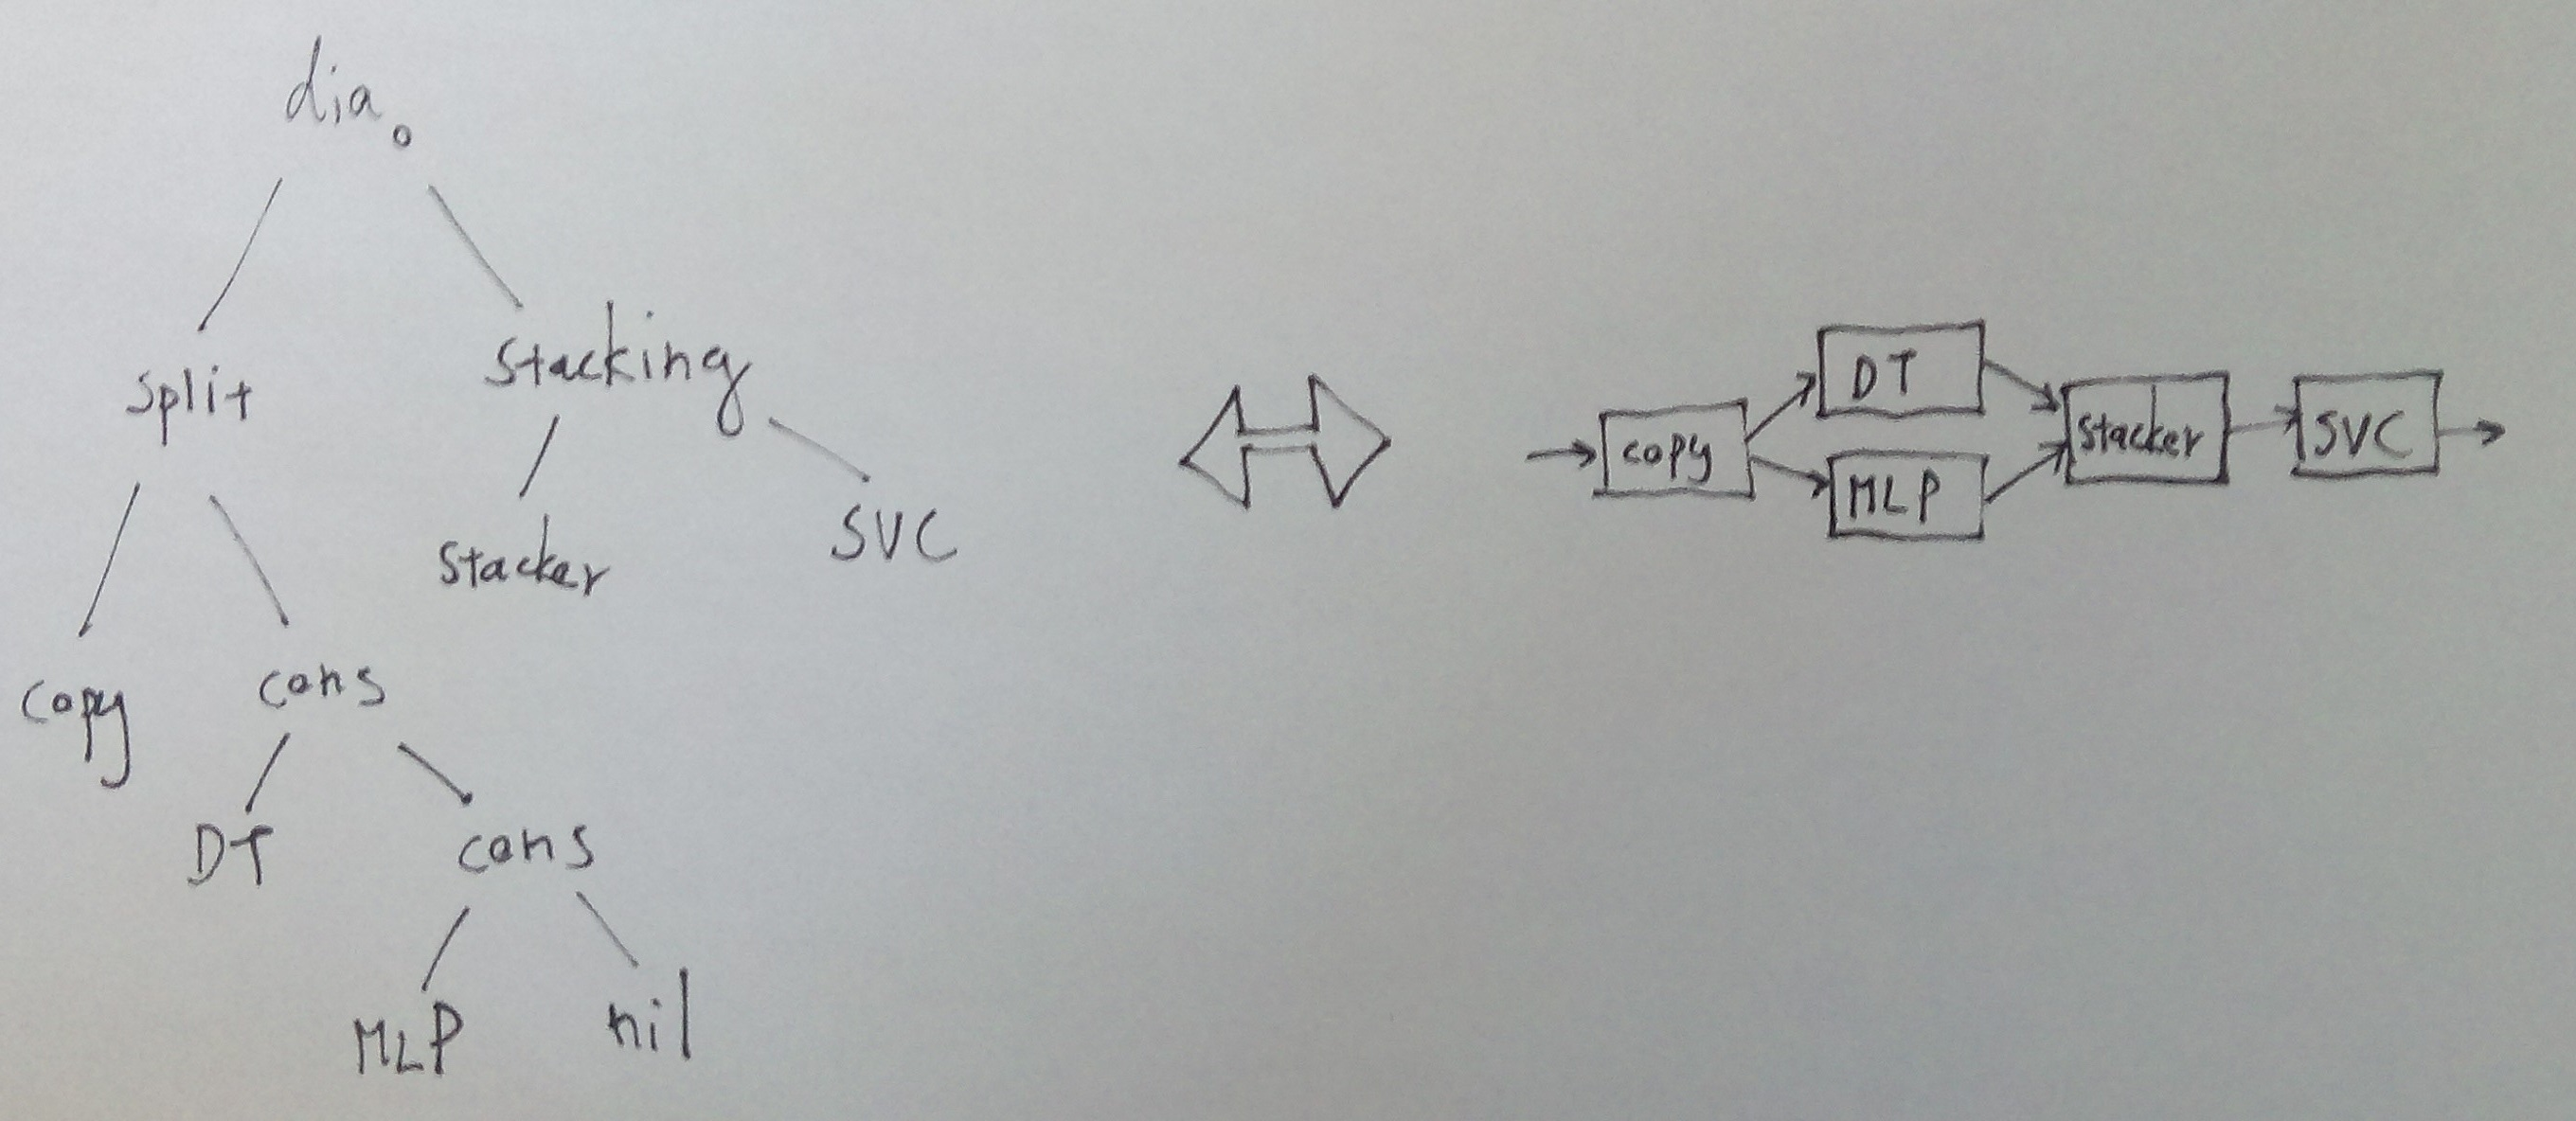
\includegraphics[width=10cm]{simple_stacking.jpg}}
\vspace*{8pt}
\caption{Simple stacking example.}
\label{simple_stacking}
\end{figure}

Although we internally use more general applicative tree representation (with all the symbols in leaf nodes),
here we present the tree as an S-expression with function symbols in the interior nodes.
Let us start in the root of the tree, where is the $dia_0$ symbol standing for DAG combinator with type:
 
$\splitter{\D}{\LD}{n}{c} \ar \merger{\LD}{\LD}{n}{c} \ar \DAG{\D}{\LD}$
  
So it is a function taking two arguments\footnote{We use the functional convention for functions with multiple arguments discussed below in the subsection about applicative notation.}, 
first of type $\splitter{\D}{\LD}{n}{c}$ and second of type $\merger{\LD}{\LD}{n}{c}$, 
and producing result of type $\DAG{\D}{\LD}$, that is a DAG with one input edge of type $\D$ and one output edge of type $\LD$ representing a classifier model.
We use names starting with uppercase letter for specific (possibly parametric) types (e.g. $\Dag, \D, \LD, \V$) 
and names starting with lowercase letter for \textit{type variables} (e.g. $n, c$).

The result of the $dia_0$ combinator is a combined classifier workflow serially composing its two arguments, which are again workflows but now with a slightly more complicated type in the middle; 
the output type of the first and the input type of the second is the same type $\Ve{\LD}{n}{c}$. 

In general $\Ve{a}{n}{c}$ is type representing a vector of $n$ values of type $a$ 
with a \textit{splitting case} $c$.
In order to explain what a \textit{splitting case} is let us have a look on the DAG of the example workflow on fig. \ref{simple_stacking}. First the input data are copied into two different classification methods and their results are prepared by stacker to by given to the SVC classifier as input data to give the final results. But if we replace the copy splitter with k-means splitter (namely 2-means since the copy to be replaced has two outputs), then the resulting workflow does not make sense any more, because models to be stacked need to be given the same data. The difference between copy and k-means is that although they have the same topology they have different approach to splitting; a copy just makes several \textit{same} copies of the input data, whereas k-means (or any clustering method in general) splits the input data into several \textit{disjoint} sub-parts. We call this splitting approach a \textit{splitting case} and distinguish two types of cases: $\Same$ and $\Disjoint$. Another thing worth mentioning is that we manage a size of a vector on the type level via the type parameter $n$.

From $dia_0 : \splitter{\D}{\LD}{n}{c} \ar \merger{\LD}{\LD}{n}{c} \ar \DAG{\D}{\LD}$ we see that
the number $n$ of output edges of the first DAG may be arbitrary but it must match the number of input edges of the second, similarly for the splitting case $c$ resulting in that stacker merger is preceded by suitable splitter. The type of $dia_0$ contains type variables which means that $dia_0$ is a \textit{polymorphic} function, i.e. it can match many specific types matching the general pattern. 
As we will go through the rest of the example we will see that the actual type of the left subtree is an instance of the type of the first parameter of the $dia_0$ combinator.




\red{TODO REST OF THE EXAMPLE}

\red{distinction of disjoint and same data vector}

\red{comment polymorphism}

We may say that our approach balances two mutually counteractive tendencies: generality and correctness. 


\subsubsection{Applicative representation of program trees}

The standard way of tree representation of tree individuals in genetic programming uses S-expressions,
i.e. an interior node represents a function with its argument sub-expressions in its direct sub-trees. 
Thus terminal symbols are in leaf nodes and function symbols are interior nodes.
On the other hand, there is a more general \textit{applicative} representation, which has all symbols in leafs and all the interior nodes are of one kind: binary explicit application operator.

This is possible thanks to the fact that all function with multiple inputs may be considered a function with one input. For example function $f : A_1 \times A_2 \ar B$ can be thought of as having type $f^\prime : A_1 \ar (A_2 \ar B)$ abbreviated as $f^\prime : A_1 \ar A_2 \ar B$. Function $f^\prime$ given a first input returns another function which given a second input returns the result of original function $f$. So instead of all at once application $f(x,y)$ we apply arguments sequentially as $f^\prime(x)(y)$. This technique is called \textit{currying}. Applicative tree representation explicitly captures those binary applications.

\red{todo obrazek toho prikladu}

The applicative representation is more general then S-expressions because now the function may be represented as an sub-expression, whereas S-expression notation allows only single symbols to act as functions (interior node can hold only a single function symbol, but not a whole expression).

With more general tree representation comes more general crossover. E.g. now the tree-swapping crossover can also swap functions, so from the S-expression point of view it can swap interior nodes, because in applicative representation all the symbols are in leafs.  

\subsection{Generating}

- Dosud jsme popsali co je cílem tvořit a co to omezuje, aby to dávalo smysl. Ted popíšem jak na to jdeme. Nejprve to ilustrujem jednoduchym prikladem to provide a context, pak formalneji predstavime general notions on which the approach is based and after that we describe the algorithm together with techniques which make it fast enough for massive use in generating and mutation.

\subsubsection{A simple example}

- to by šlo snad názorně ukázat na příkladě generování stromu k>1:
- Generujem Dag D LD, k>1 -> v kořeni stromu je aplikace tedy:
- levej syn je funkce z něčeho do (Dag D LD), pravej syn je to něco
… az se dostanem do listů (strom velikosti 1) - výběr symbolu z gammy aby to pasovalo..

\subsubsection{Existential queries}

- 1. základ našeho přístupu: ex. sigma že z gamma de vyvodit že M je typu sigma(tau)
  - k tomu je potřeba definovat prerekvizitní pojmy, minimálně tyto:
    - substituce
    - a to jakym způsobem vypadá dotaz (k,tau) - a že je teda obecnejší to tau než přímo typ že pak M:Tau

to kulminuje v hodící se funkci subs, která pro danej dotaz (k,tau) vrátí substituce spolu s počtama stromů


\subsubsection{Generating based on sizes}

- 2. základ našeho přístupu: generuje strom pro danou velikost stromu (počet symbolů).
  - což mimojiné umožnuje mnohem přímější kontrolu nad tím, z jakého rozložení taháme naše jhedince 
  - zde popsat to jak to děláme (32, 16,16, 8,8,8,8, ...)

\subsubsection{Counting the trees}

- 2. základ našeho přístupu: počítáme si počty stromů pro jednotlivý dotazy 
     - abychom byli schopný generovat (semi-)uniformě

\subsubsection{Final overview of generating}

- pridáme skolemizaci aby to fungovalo
- kesování aby se dalo generovat rychle
    - předpočítání pomocných dat pro generování
    - "semi-unfiromní" generování - pozn o nedokonalosti 
- kulminující v pseudokódu


\newcommand{\nv}{v}
\newcommand{\ball}{\op{treeID}}

\Pseudokod{Get tree individual of size 1.}
{\textbf{getTree$_1$}($\tau$, $\ball$, $\nv_0$)}{
	\For {$(s,\tau_s) \in \Gamma$}{
		$(\tau_s^{\prime},\nv_1) \la fresh_\tau(\tau_s,\nv_0)$ \;
		\If {$\exists ~ \mu = \mgu{\tau,\tau_s^{\prime}}$} {
			\If {$\ball = 0$} {
				\Return $(s:\mu(\tau), \nv_1)$
			} \Else {
				$\ball \la \ball - 1$				
			}
		}	
	}
}{genOne1}

\Pseudokod{Get tree individual of size $k > 1$.}
{\textbf{getTree$_k$}($\tau$, $\ball$, $\nv_0$)}{
	\For {$i \in \{1,\dots,k-1\}$}{
		$j \la k - i$ \;
		$(\alpha, \nv_1) \la newVar(\tau,\nv_0)$ \;
		\For {$(n_F,\sigma_F,\nv_2) \in subs_i(\alpha \ar \tau, \nv_1 )$}{
			\For {$(n_X,\sigma_X,\nv_3) \in subs_j(\sigma_F(\alpha), \nv_2 )$}{
				$n_{FX} \la n_F \cdot n_X $ \;
				\If {$\ball < n_{FX}$} {
					\textbf{random} $\ball_F \in \{0,\dots,n_F - 1\}$ \;
					\textbf{random} $\ball_X \in \{0,\dots,n_X - 1\}$ \;					
					$(F, \nv_4)  \la getTree_i(\overline{\sigma_F(\alpha \ar \tau)}, \ball_F,\nv_3)$ \;
					$(X, \nv_5) \la getTree_j(\overline{\sigma_X(\sigma_F(\alpha)}), \ball_X,\nv_4)$ \;
					\Return $((F~X) : \sigma_X(\sigma_F(\tau)), \nv_5)$				
				} \Else {
					$\ball \la \ball - n_{FX}$				
				}			
			}
		}	
	}
}{genOneK}



\section{Experiments}

In this section, we describe the experiments we performed in order to evaluate
the quality of GP-ML. The algorithm is compared to a baseline, which consists of
the performance of all the methods used in the ensembles with tuned parameters.
We also compare the current version of GP-ML to its two previous
versions\cite{SSCI2015,7814654}.

\subsection{Description}

We performed extensive testing of the GP-ML algorithm on four datasets from the
UCI machine learning repository\cite{Lichman:2013}. These are 
winequality-white\cite{Cortez2009547} (referred to as `wine' in the rest of the paper),
wilt\cite{Johnson:2013:HPA:2512892.2512894}, magic\cite{Bock2004511},  and ml-
prove\cite{Bridge}. The datasets come from different areas and have  different
interesting features. In the wine dataset, the goal is to predict  the quality
of white wine on a scale 1-9 based on its chemical and physical  properties. The
wilt dataset aims to classify images into two classes based on features from
different image analysis approaches. The magic dataset contains  data from the
field of particle physics -- the goal is to predict whether an observation is a
gamma particle or not. Finally, the ml-prove dataset contains information on
different tasks from automated theorem proving. The goal is to  predict which
automated provers would perform the best for each task. The wine and wilt
datasets both contain about 5,000 instances. The wine dataset has 11 attributes
and the wilt dataset has 6 attributes. The other two datasets are larger -- 
ml-prove has over 6,000 instances with 51 attributes and magic has more than 
19,000 instances with 10 attributes.

All the machine learning workflows consists of different types of techniques. We
used principal component analysis (PCA) and the selection of $k$ features most
correlated with the target ($k$-best) as preprocessing techniques. We also used
$k$-means as a data splitting technique -- instances from different clusters are
treated separately in the workflow. A copy operator which copies the same
instances to multiple parts of the workflow is also present. In the two oldest
versions of GP-ML we used support vector classification (SVC), logistic
regression (LR), gaussian naive Bayes classifier (GNB), and decision trees (DT)
as the basic machine learning techniques. In the current version of GP-ML we
also added perceptron (Perc), linear discriminant analysis (LDA), quadratic
discriminant analysis (QDA), passive aggressive classifier (PAC), SGD classifier
(SGD), and multi-layered perceptron (MLP) to the set of available base
classifiers. In GP-ML-v1, voting is the only ensemble technique supported.
Versions 2 and 3 additionally support stacking and boosting ensembles. In these
ensembles, the outputs of sub-workflows are combined in order to obtain the 
result of the whole ensemble.

Many of the machine learning methods mentioned in the previous paragraph have a
number of hyper-parameters which need to be set correctly in order to achieve
the optimal performance. For each of these parameters, we selected a range of
suitable values and the genetic programming evolved the values of the parameters
together with the whole workflow. All the possible values of the parameters for
those methods that have any parameters are presented in
Table~\ref{tab:hyperparameters}. We used the implementation from the scikit-learn 
library and all parameters not mentioned here use their default values.

\begin{table}
\tbl{The possible values of hyper-parameters for the machine learning methods. 
\label{tab:hyperparameters}}
{\begin{tabular}{ll}
\hline
\multicolumn{2}{c}{Support Vector Classifier} \\
\hline
C & \{0.1, 0.5, 1, 2, 5, 10, 15\} \\
gamma & \{0.0, 0.0001, 0.001, 0.01, 0.1, 0.5\} \\
tol & \{0.0001, 0.001, 0.01\} \\
\hline
\multicolumn{2}{c}{Logistic Regression (penalty=l2, solver=sag)} \\
\hline
C & \{0.1, 0.5, 1, 2, 5, 10, 15\} \\
tol & \{0.0001, 0.001, 0.01\} \\
\hline
\multicolumn{2}{c}{Decision Tree Classifier} \\
\hline
criterion & \{gini, entropy\} \\
max\_features & \{0.05, 0.1, 0.25, 0.5, 0.75, 1\} \\
max\_depth & \{1, 2, 5, 10, 15, 25, 50, 100\} \\
min\_samples\_split & \{1, 2, 5, 10, 20\} \\
min\_samples\_leaf & \{1, 2, 5, 10, 20\} \\
\hline
\multicolumn{2}{c}{Perceptron} \\
\hline
penalty & \{'None', 'l2', 'l1', 'elasticnet'\} \\
n\_iter  & \{1, 2, 5, 10, 100\} \\
alpha & \{0.0001, 0.001, 0.01\} \\
\hline
\multicolumn{2}{c}{SGD} \\
\hline
penalty & \{'none', 'l2', 'l1', 'elasticnet'\} \\
loss & \{'hinge', 'log', 'modified\_huber', 'squared\_hinge', 'perceptron'\} \\
n\_iter & \{5, 10, 100\} \\
alpha & \{0.0001, 0.001, 0.01\} \\
l1\_ratio & \{0, 0.15, 0.5, 1\} \\
epsilon & \{0.01, 0.05, 0.1, 0.5\} \\
learning\_rate & \{'constant', 'optimal'\} \\
eta0 & \{0.01, 0.1, 0.5\} \\
power\_t & \{0.1, 0.5, 1, 2\} \\
\hline
\multicolumn{2}{c}{PAC} \\
\hline
loss & \{'hinge', 'squared\_hinge'\} \\
C & \{0.1, 0.5, 1.0, 2, 5, 10, 15\} \\
\hline
\multicolumn{2}{c}{LDA} \\
\hline
solver & \{'lsqr', 'eigen'\} \\
shrinkage & \{None, 'auto', 0.1, 0.5, 1.0\} \\
\hline
\multicolumn{2}{c}{QDA} \\
\hline
reg\_param & \{0.0, 0.1, 0.5, 1\} \\
tol & \{0.0001, 0.001, 0.01\} \\
\hline
\multicolumn{2}{c}{MLP} \\
\hline
activation & \{'identity', 'logistic', 'relu'\} \\
solver & \{'lbfgs', 'sgd', 'adam'\} \\
alpha & \{0.0001, 0.001, 0.01\} \\
learning\_rate & \{'constant', 'invscaling', 'adaptive'\} \\
tol & \{0.0001, 0.001, 0.01\} \\
max\_iter & \{10, 100, 200\} \\
learning\_rate\_init & \{0.0001, 0.001, 0.01\} \\
power\_t & \{0.1, 0.5, 1, 2\} \\
momentum & \{0.1, 0.5, 0.9\} \\
hidden\_layer\_sizes & \{(100,), (50,), (20,), (10,)\} \\ 
\hline
\multicolumn{2}{c}{PCA} \\
\hline
whiten & \{true, false\} \\     
n\_components & \{$\lfloor k \cdot N \rfloor | k \in$ \{0.01, 0.05, 0.1, 0.25, 0.5, 0.75, 1\} \\
\hline
\multicolumn{2}{c}{kBest} \\
\hline
k & \{$\lfloor k \cdot N \rfloor | k \in$ \{0.01, 0.05, 0.1, 0.25, 0.5, 0.75, 1\} \\
\hline
\end{tabular}}
\end{table} 

We used the quadratic weighted $\kappa$ as the metric for the evaluation in all
the datasets except magic. The quadratic weighted $\kappa$ expresses how well a
classifier agrees with the ground truth. It is especially suited for grading
tasks (wine) or binary classification tasks where one of the classes are much
less common than the other one. The values of $\kappa$ are always between -1 and
1, where 1 means complete agreement between the classifier and the ground truth,
-1 means  compete disagreement and 0 is as  good as random guessing. For the
magic dataset, we used the accuracy as the metric optimized by GP-ML, because
the problem has five classes which have no ordering and thus, the $\kappa$
values would make no sense. All values presented in this paper are results of
five fold cross-validation. Moreover, the GP-ML results averages of five
independent runs.

The new technique for generating individuals enables the newest version of 
GP-ML to work with larger trees, therefore some of the parameters described
bellow are different for this version compared to the previous versions.

All version of GP-ML first generate 256 individuals with maximum size of 20 (GP-
ML v1 and v2) or 64 (GP-ML v3). Once at least 64 of them are evaluated, after
each evaluation a new individual is created using the genetic operators, and
once the population size is more than 512 individuals, the worst individual is
discarded from the population. The offspring are created by a typed crossover
(probability 0.4), subtree mutation (probability 0.3), or single parameter
change mutation (probability 0.3). The typed crossover randomly exchanges two
subtrees of the same type in two individuals. The maximum size of tree after
crossover is 128 nodes for GP-ML v3 and 50 for the older versions. The subtree
mutation generates a random subtree of at most 32 nodes (20 nodes for GP-ML v1
and v2).

The evolution run for 32,768 evaluations for the wilt and wine datasets, 17,920
evaluations for the ml-prove dataset and 7,680 for the magic dataset.
Additionally, the GP-ML v3 was stopped after 5 hours on the wilt dataset and
after 10 hours on the other datasets. The runs for this version were performed
on 16 CPUs each. The time-based stopping is important as sometimes the fitness
evaluations can be very long and running the algorithm until it reaches the 
predefined number of evaluations may be impractical.

\subsection{Results}

The results of the experiments are shown in Table~\ref{tab:results}. It shows
the quadratic weighted $\kappa$ (all datasets except magic) or accuracy (magic).
For the simple methods (except MLP), we used an exhaustive grid search in order
to test all the combinations of parameters from Table~\ref{tab:hyperparameters}
and show the best result obtained. The MLP has a large number of parameters and
therefore there is a large number of different settings (more than 100,000),
moreover, MLPs are quite slow and therefore we were not able to perform the full
grid search for MLP. Instead, we run a random search and tested many different
combinations of the parameters.

\begin{table}
\tbl{Comparison of the results of parameter tuning (grid search for most 
methods, random search for methods marked by $+$) for the base methods with the
results of the three versions of GP-ML on the four datasets. Average quadratic 
weighted $\kappa$ for all datasets except magic, and accuracy for the magic 
dataset. \label{tab:results}}
{\begin{tabular}{lllll}
\toprule
method 						& magic 	& ml-prove 	& wilt 		& wine      \\
\colrule
DT 							& 0.6622 	& 0.5116 	& 0.8060 	& 0.4477    \\
GNB 						& 0.3289	& 0.1696 	& 0.2917 	& 0.4206    \\
LDA 						& 0.5395 	& 0.4499 	& 0.5112 	& 0.4405    \\
LR 							& 0.4880 	& 0.4523 	& 0.0148 	& 0.1414    \\
							% 6900		  11070		  32200		  27830
MLP 						& 0.6189$^+$& 0.5304$^+$& 0.7700$^+$& 0.3832$^+$\\
PAC 						& 0.3017 	& 0.3704 	& 0.2504 	& 0.1385    \\
Perc 						& 0.4523 	& 0.3730 	& 0.2441 	& 0.1758    \\
QDA 						& 0.4792    & 0.3297 	& 0.8217 	& 0.4918    \\
SGD 						& 0.5128 	& 0.4608 	& 0.4513 	& 0.3840    \\
SVC 						& 0.6147	& 0.5361 	& 0.8416 	& 0.3224    \\
\colrule
GP-ML v1\cite{SSCI2015} 	& 0.7084 	& 0.5689 	& 0.8702 	& 0.4792    \\
GP-ML v2\cite{7814654} 		& 0.7113	& 0.5779	& 0.8858 	& 0.4982    \\
GP-ML v3					& 0.7084	& 0.5638	& 0.8913	& 0.5146    \\			
\botrule
\end{tabular}}
\end{table} 

\section{Conclusion and Future Work}

\section*{Acknowledgments}

Martin Pil\'{a}t and Roman Neruda have been supported by Czech Science
Foundation project no.~P103-15-19877S. Tom\'a\v{s} K\v{r}en has been supported
by the Grant Agency of the Charles University project no.~187115 and by SVV
project number 260~333.

Access to computing and storage facilities owned by parties and projects
contributing to the National Grid Infrastructure MetaCentrum, provided under the
programme "Projects of Large Research, Development, and Innovations
Infrastructures" (CESNET LM2015042), is greatly appreciated.

\bibliographystyle{ws-ijait}
\bibliography{sample}

\end{document} 
